\documentclass[a4paper,10pt]{article}
%\documentclass[preview=false]{standalone}
% %%%% Define new conditional \ifplastex
% %%%% This ensure that the file complied normally without plasTeX.
\usepackage{plastex}

\usepackage{hyperref}

\ifplastex\else
\usepackage{standalone} %%%% Only load standalone when not in plasTeX
\standalonetrue
\usepackage{longtable} %%%% Only load longtable and ltcaption when not in plasTeX
\usepackage{ltcaption}
\fi

% Package for typesetting URLs
\usepackage{url}

% Package for including graphics.
\usepackage{graphicx}

\usepackage{multicol}

\usepackage{bsymb}

% Package for typesetting Event-B models
\usepackage[colour]{eventB}
%\usepackage{eventB-vhdl}

% Package for typesetting dates and times
\ifplastex
\newcommand{\SCManualDate}{May 12th, 2020}
\else
\usepackage{datetime}
\newdate{SCManualDate}{27}{7}{2017}
\fi
\newcommand{\SCFeatureVersion}{0.0.0}
\newcommand{\SCManualVersion}{0.0.0}

% Title
\title{Scenario Checker User Manual} 

% Author
\author{%s
  Dr Colin Snook\\%
  ECS, University of Southampton\\%
  \texttt{\href{mailto:cfs@soton.ac.uk}{cfs at soton dot ac dot uk}}%
}%


% Date
\date{%
  Version \SCManualVersion\\%
  (for feature version \SCFeatureVersion)\\
  \ifplastex
  \SCManualDate
  \else
  \displaydate{SCManualDate}%
  \fi
}

\begin{document}
\ifplastex%
\maketitle% Make title if in plasTeX mode.
\else%
 \ifstandalone%
 \maketitle % Make title if in standalone mode.
 \else%
 \fi%
\fi%

\section{Overview}
\label{sec:overview}

The Scenario Checker is a tool to help develop useful Event-B models.
The Scenario Checker focusses on a behaviour-driven approach to validate model behaviour.
The Scenario Checker does not verify that models are consistent: Rodin automatic provers should be used to verify models.
The Scenario Checker uses the ProB animator to execute the model.

The Scenario Checker allows scenarios to be animated and recorded while visualising the state of variables and enabledness of events in the model.
When the model has been modified, scenarios can then be re-played to check for changes.

It is assumed that part of the model represents a controller and other parts represent the controlled devices in the environment.
Events designated as internal steps of the controller are run automatically until completion (i.e. until no more internal events are enabled) and private variables of the controller are ignored.
Events may also be prioritised to resolve non-deterministic choices remaining in the model.

\subsection{Release Notes}
\label{sec:release-notes}

\begin{itemize}
	\item \textbf{0.0.0} - prototype release
\end{itemize}

\subsubsection{Known Issues}
\label{sec:known-issues}

\begin{itemize}
	\item using the small step button in playback can result in errors
\end{itemize}


%%% Local Variables:
%%% mode: latex
%%% TeX-master: "user_manual"
%%% End:


\section{Getting Started}
\label{sec:getting-started}

\subsection{Setup}
\label{sec:setup}

The Scenario Checker is installed into Rodin from the plugin update site in the normal way.
It is located under the Utilities category.

The Scenario Checker depends on (and will install elements from)
\itemize{
\item ProB - de.prob
\item ProB Support - ac.soton.eventb.probsupport
\item Event-B EMF framework - org.eventb.emf
\item Oracle - persistence for scenarios
}

\subsection{Perspective}
\label{sec:perspective}

The Scenario Checker defines a perspective (see Fig. \ref{fig:perspective}) which includes the Scenario Checker Control Panel view and the Scenario Checker State view.
The perspective also includes the ProB History view which is used to see the executed scenario (including internal events). 
The ProB State view is also included (stacked behind Scenario Checker State) in case a more detailed view of state is needed.

\begin{figure}[!htbp]
	\centering
	\ifplastex
	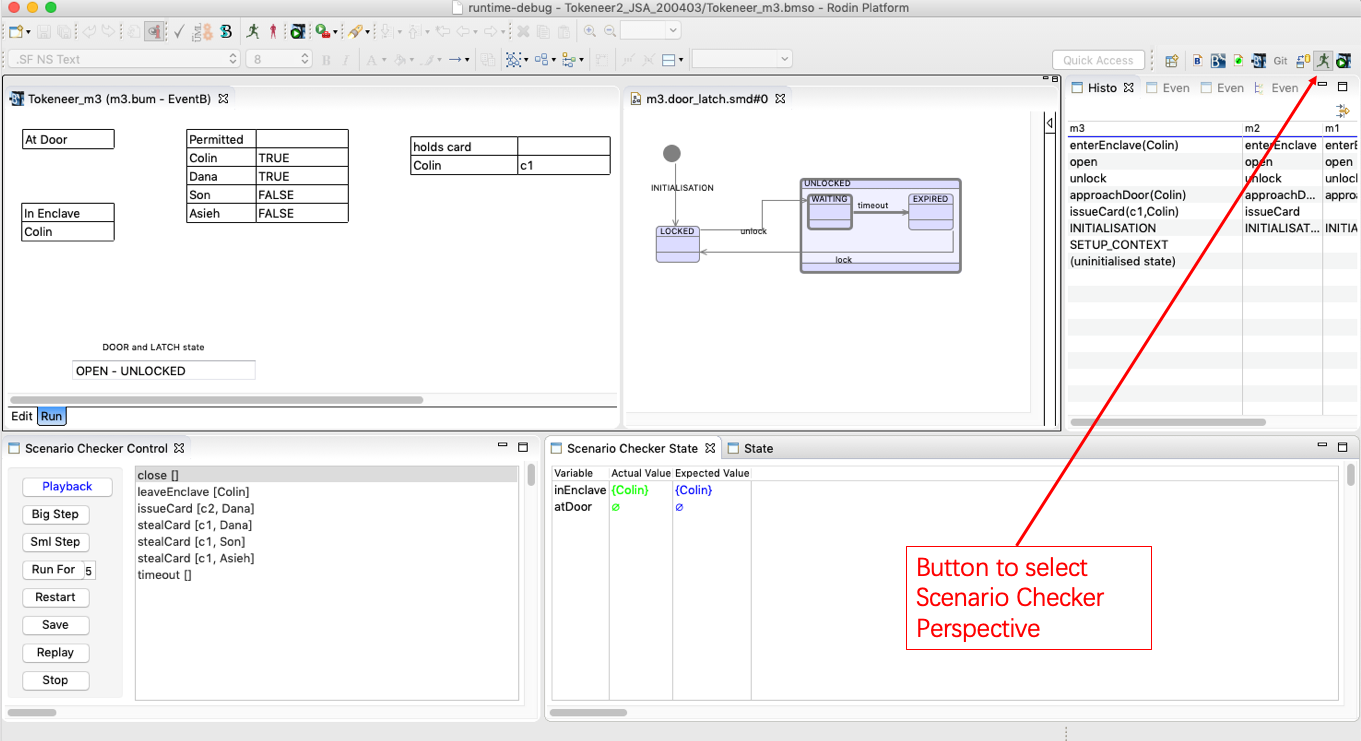
\includegraphics[width=900]{figures/perspective}
	\else
	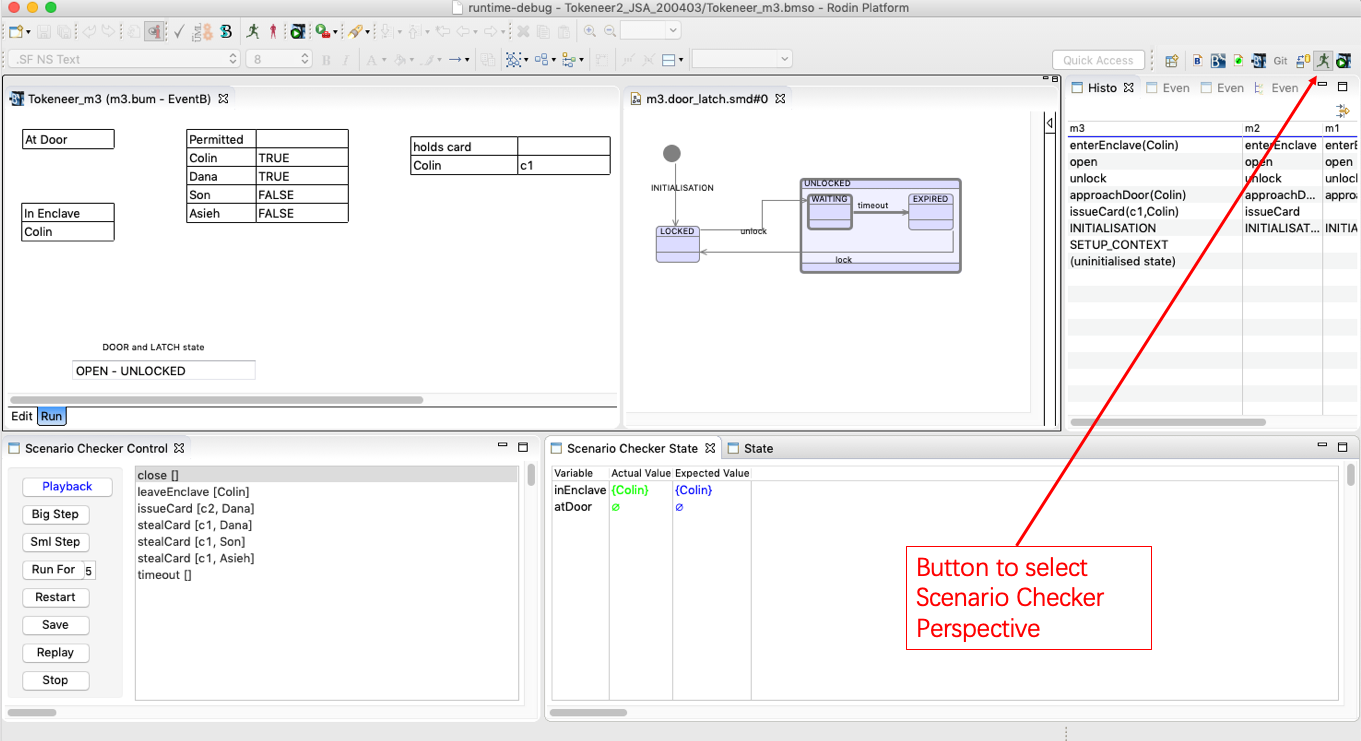
\includegraphics[width=0.9\textwidth]{figures/perspective}
	\fi
	\caption{Scenario Checker Perspective}
	\label{fig:perspective}
\end{figure}

The Scenario Checker views are also contributed to the BMotion Studio Run perspective and are available as short cuts on the Event-B perspective.

\subsection{Starting}
\label{sec:starting}

The Scenario Checker is started using the context menu of a machine as shown in Fig. \ref{fig:starting1}.
I.e. by right clicking on a machine in the Event-B navigator and selecting the \textbf{Scenario Checker} menu item.

\begin{figure}[!htbp]
	\centering
	\ifplastex
	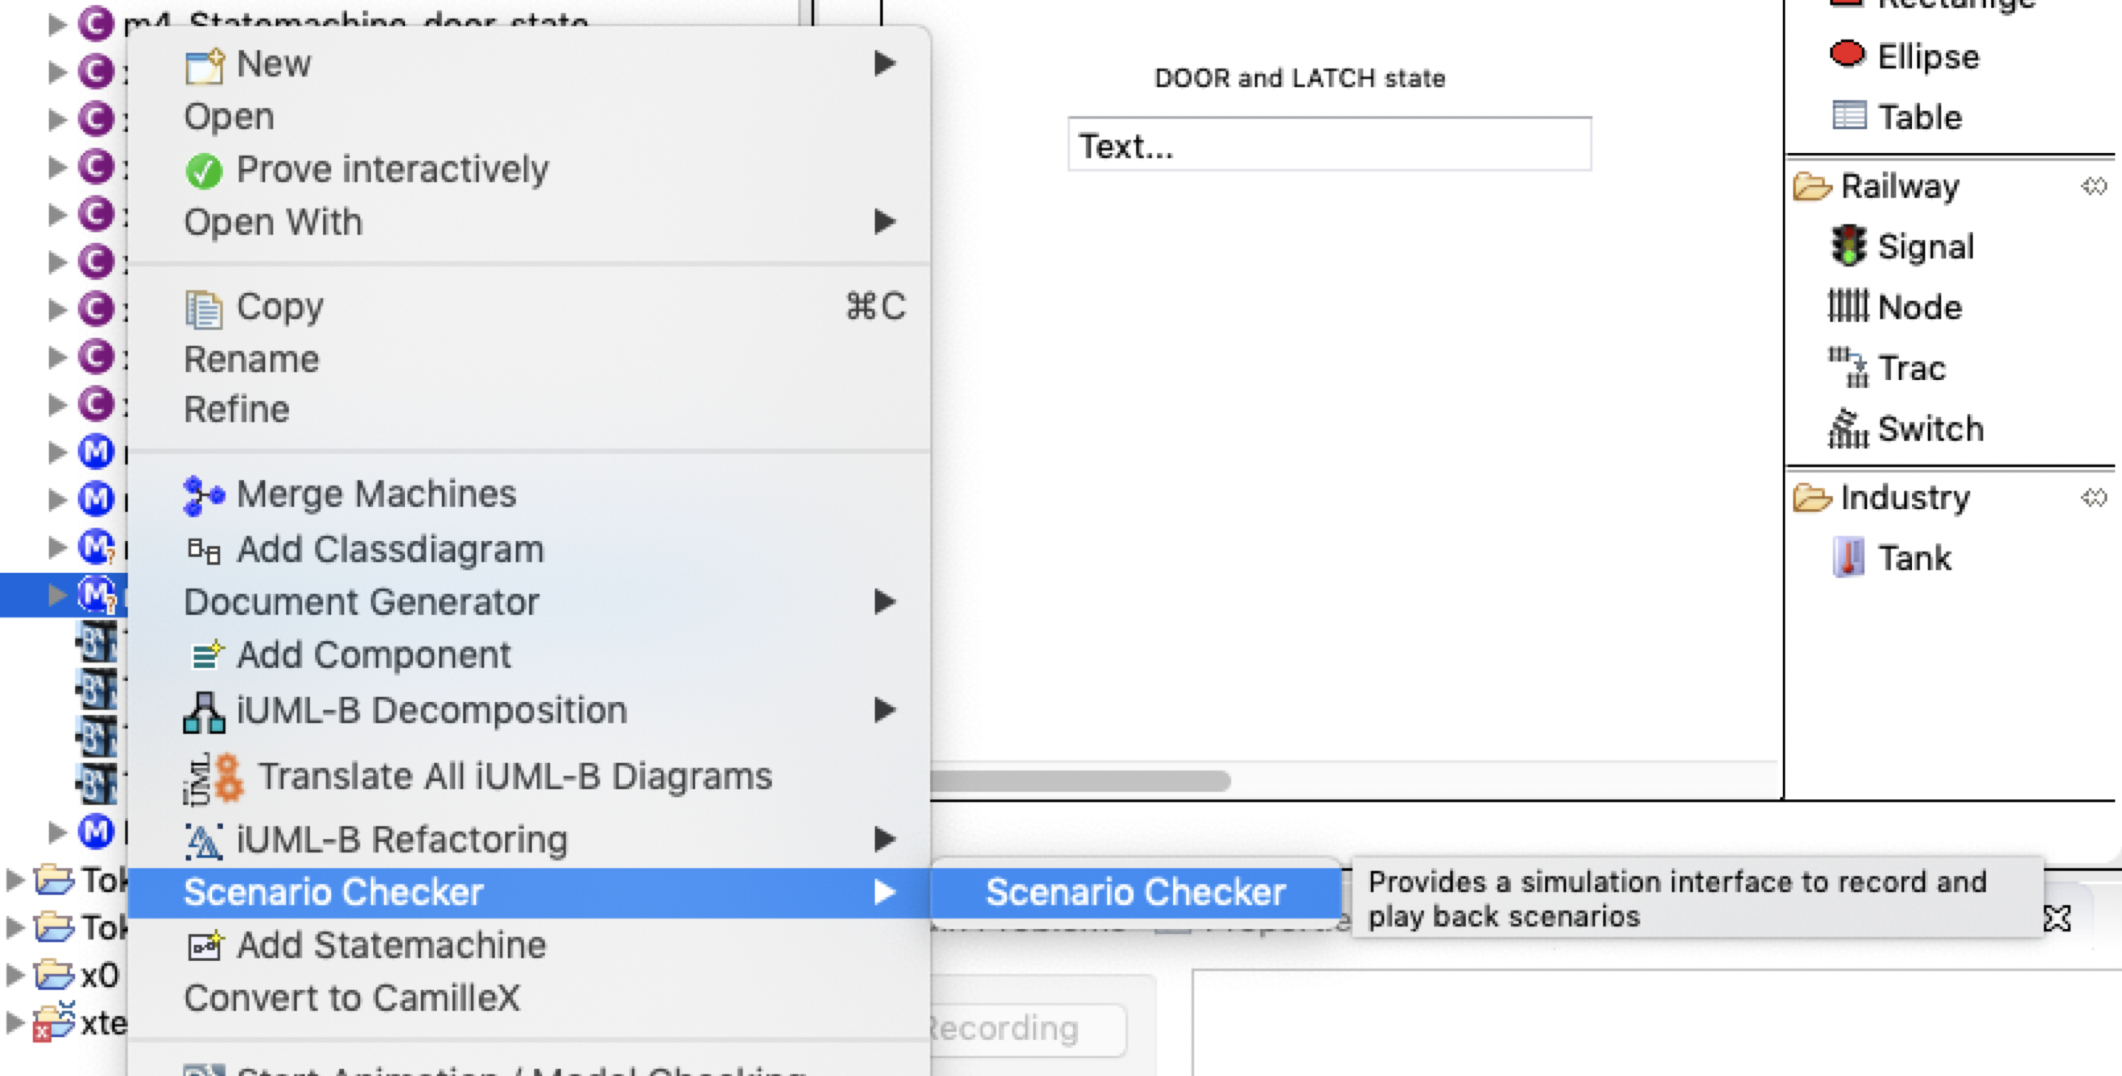
\includegraphics[width=700]{figures/starting1}
	\else
	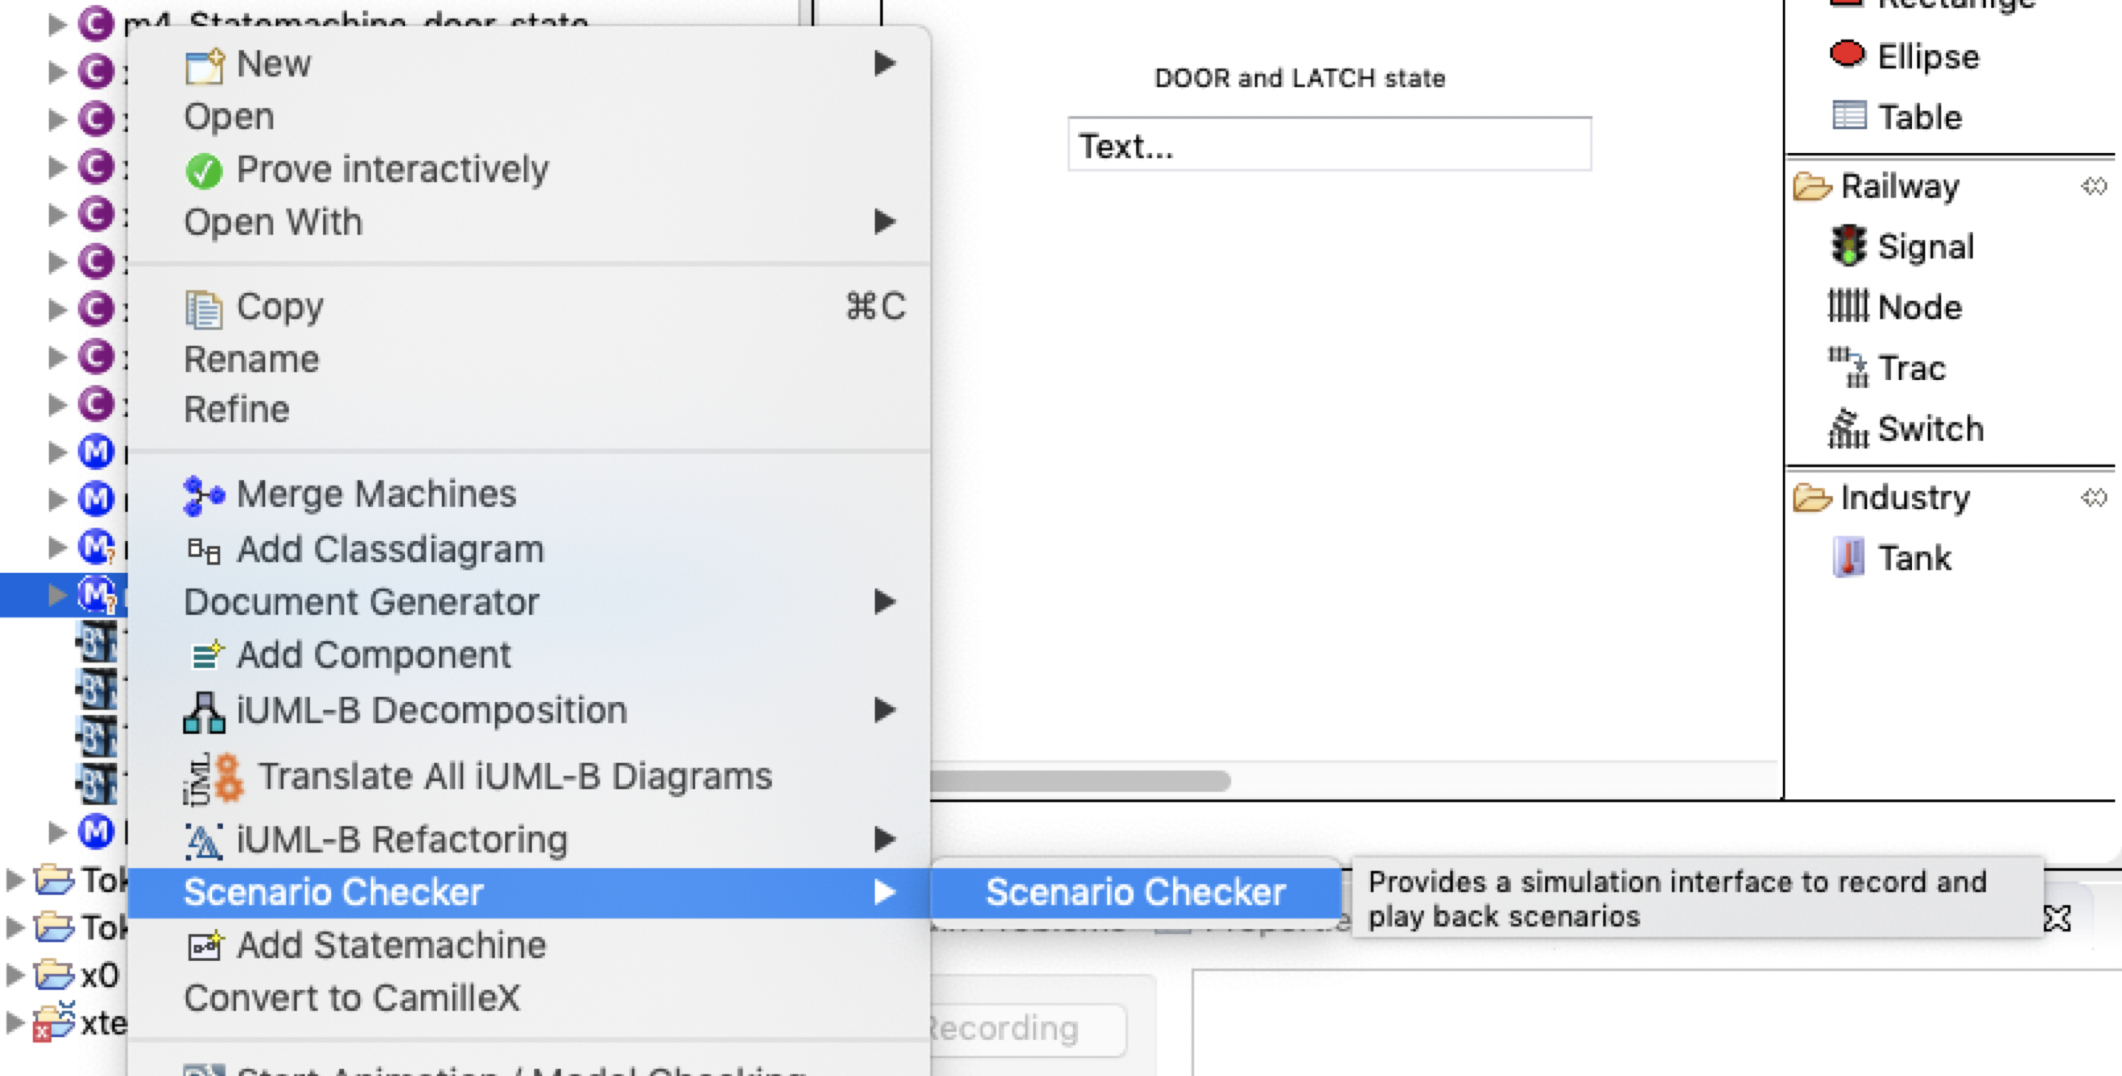
\includegraphics[width=0.75\textwidth]{figures/starting1}
	\fi
	\caption{Starting the Scenario Checker from the context menu}
	\label{fig:starting1}
\end{figure}

An alternative way to start the Scenario Checker is to ensure that at least one of the scenario views is opened (e.g. by selecting the Scenario Checker perspective) and then using the toolbar button of the ProB support plug-in (the green running man shown circled in red in \ref{fig:starting2}).

\begin{figure}[!htbp]
	\centering
	\ifplastex
	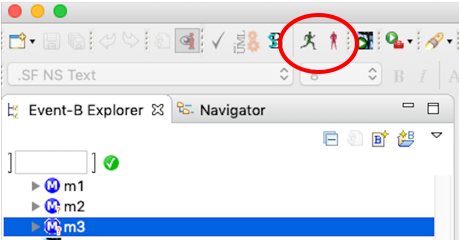
\includegraphics[width=400]{figures/starting2}
	\else
	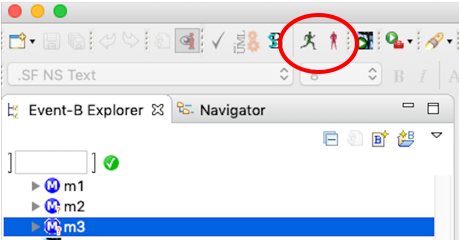
\includegraphics[width=0.4\textwidth]{figures/starting2}
	\fi
	\caption{Starting/Stopping the Scenario Checker using the toolbar icons}
	\label{fig:starting2}
\end{figure}

In either case, the ProB support plug-in will be used to simultaneously launch the scenario checker and any other participating animation plugins that are open for  the same machine.
For example, a BMotion Studio visualisation and/or a UML-B state-machine could be used to visualise the state of the model to assist validation.

The Scenario Checker should be stopped by selecting the machine again and using the red standing man toolbar button.

Warning: If another animation is started using the ProB support plugin, any current animation will be aborted.

\subsection{Setup}
\label{sec:setup}

The Scenario Checker always fires the ProB setup operation whenever it can (i.e. when it is started or re-started or replayed).
It is important for the sets and constants in the model, to be instantiated with suitable values to record a desired scenario.
The same values must also be instantiated in order for previously recorded scenarios to be replayed.
This can be done by adding an animation context that is seen by the machine to be animated.

\subsection{Persistence}
\label{sec:persistence}

Scenarios are persisted in the Oracle format.
This is an XML based format consisting of two types of elements (Steps and Snapshots) which are expected to alternate.
A \textbf{Step} records the event signature that fired as part of the scenario.
A \textbf{Snapshot} records the state of any variables and constants that changed value as a result of the preceding step.
The first step is always the ProB \texttt{SETUP} operation and this is followed by the first snapshot giving the values of sets and constants.
The second step is the \texttt{INITIALISATION} followed by the snapshot giving the initial value of all variables.
After this the steps and snapshots depend on the scenario.
The oracle format is defined and generated from an EMF meta-model and hence is the default EMF XMI format for that meta-model.
Scenarios can be read and edited using an EMF editor such as Rose.


%%% Local Variables:
%%% mode: latex
%%% TeX-master: "user_manual"
%%% End:


% !TEX root = user_manual.tex

\section{Concepts}
\label{sec:concepts}

The Scenario Checker is based on the following concepts:
\begin{itemize}
		\item A model represents a closed system involving a controller and the sensed and controlled environment.
		\item A scenario consists of a sequence of external events that occur in the sensed environment. 
		\item After each external event, a resulting state is expected.
		\item The model of the controller may include internal events which are not specified in the scenario. 
		Events in the model may be designated as internal by adding a generic boolean attribute, Internal=true, or inserting <INTERNAL> in the comment property.
		\item The model of the controller may include private variables which are not specified in the scenario.
		Variables in the model may be designated as private by adding a generic boolean attribute, Private=true, or inserting <PRIVATE> in the comment property.
		\item Events may be given a priority to add control of ordering of events when this is not specified by the model. 
		Event priority is given by adding a generic integer attribute, Priority=n, or inserting <PRIORITY=n> in the comment property, where n is a natural number.
		(Low priority numbers are executed first).
		Note that prioritising events results in validating a particular refinement of the actual model.
\end{itemize}
	
The Scenario Checker provides:
\begin{itemize}
	\item A Control Panel to control the execution of external events, recording and playback of scenarios, and to view the enabled external events.
	\item A State View to monitor the value of variables and to indicate differences from the expected values.
\end{itemize}


%%% Local Variables:
%%% mode: latex
%%% TeX-master: "user_manual"
%%% End:


\section{Tasks}
\label{sec:tasks}

The Scenario Checker has two modes: Recording and Playback. 
The current mode is indicated by the label at the top of the control panel (see Figs.~\ref{fig:recording} and \ref{fig:playback}) 

The Scenario Checker is always started in the recording mode.
It changes to playback mode when the Replay button is pressed.
It changes to recording mode when the Stop button is pressed or automatically when the scenario is completed (has no more steps).

\subsection{Recording a Scenario}
\label{sec:recording}

With the Scenario Checker in recording mode, the user can choose from the available external events and arguments that are listed in the Scenario Checker Control Panel (see lower left view in Fig.~\ref{fig:recording}). 
The chosen  event is executed (either by double clicking on it, or selecting it and then pressing the Big Step button).
The Scenario Checker automatically runs internal events until completion and then updates the Scenario Checker State view to show the state of all non-private variables.

At any point, after firing a sequence of events, the scenario can be saved without altering the current scenario execution. 
This makes it easy to record intermediate points in a scenario.
The ProB history view can be used to return to any point in the scenario history.
For example if the user makes a mistake or decides that a different event trace would have been better, the ProB History view can be used to discard the later part of the trace and a new sequence can be continued from that point on.
(Note that, when saving, the scenario execution is always obtained from ProB's animation history, rather than any user interaction with the Scenario Checker).

In recording mode, the Scenario Checker Control Panel buttons have the following function:
\begin{itemize}
	\item \textbf{Big Step}  Executes events until completion of the next big step. If an operation has been selected from the list of enabled external events in the Scenario Checker Control Panel (by single clicking on it), that event will be executed. If no such event is selected, one will be picked at random. In either case, if after executing the external event any internal events are enabled, one will be executed at random and according to any priority that has been defined in the model (see Section~\ref{sec:concepts}). Firing of internal events will continue in this way until none are enabled or a loop is detected. (A loop is detected when the same event has already been executed in this run to completion). Double clicking on an event in the list of enabled events in the Scenario Checker Control Panel is exactly the same as selecting the event and using the big step button.
	\item \textbf{Small Step}  Executes one event which is selected as follows. If an operation has been selected from the list of enabled external events in the Scenario Checker Control Panel (by single clicking on it), that event will be executed. Otherwise, if any internal events are enabled, one will be executed at random and according to any priority that has been defined in the model (see section~\ref{sec:concepts}). Note that it is possible to ignore internal events using the small step button which may lead to scenarios that fail when played back (since it is not usual behaviour to ignore internal events).
	\item \textbf{Run For..}  Executes the number of big steps shown in the text box next to the button. The number can be changed by clicking in the box and editing the number.
	\item \textbf{Restart}  Discards the current scenario and restarts animation from the INITIALISATION. If the scenario had progressed beyond the INITIALISATION event, a warning and confirmation message box is displayed.
	\item \textbf{Save}  Saves the current scenario and continues without interruption. This enables common prefixes to be saved as partial scenarios for later completion. The scenario is saved in a folder called `Oracle' inside the Event-B project. The filename is automatically constructed from the machine name and a timestamp with the extension, `oracle'.
	\item \textbf{Replay}  Switches to playback mode and allows the user to select a previously recorded scenario oracle file to play. This discards the current scenario after a warning confirmation from the user.
	\item \textbf{Stop}  Has no effect in recording mode.
\end{itemize}

In recording mode, if the scenario has progressed beyond INITIALISATION (i.e. there is a useful scenario that could be saved) the Scenario Checker Control Panel indicates that a scenario could be saved by displaying an asterix (`*') in the title bar.

In recording mode the Scenario Checker View displays the current value of all non-private variables irrespective of whether they have changed or not.
The Expected value column is left blank.

\begin{figure}[!htbp]
	\centering
	\ifplastex
	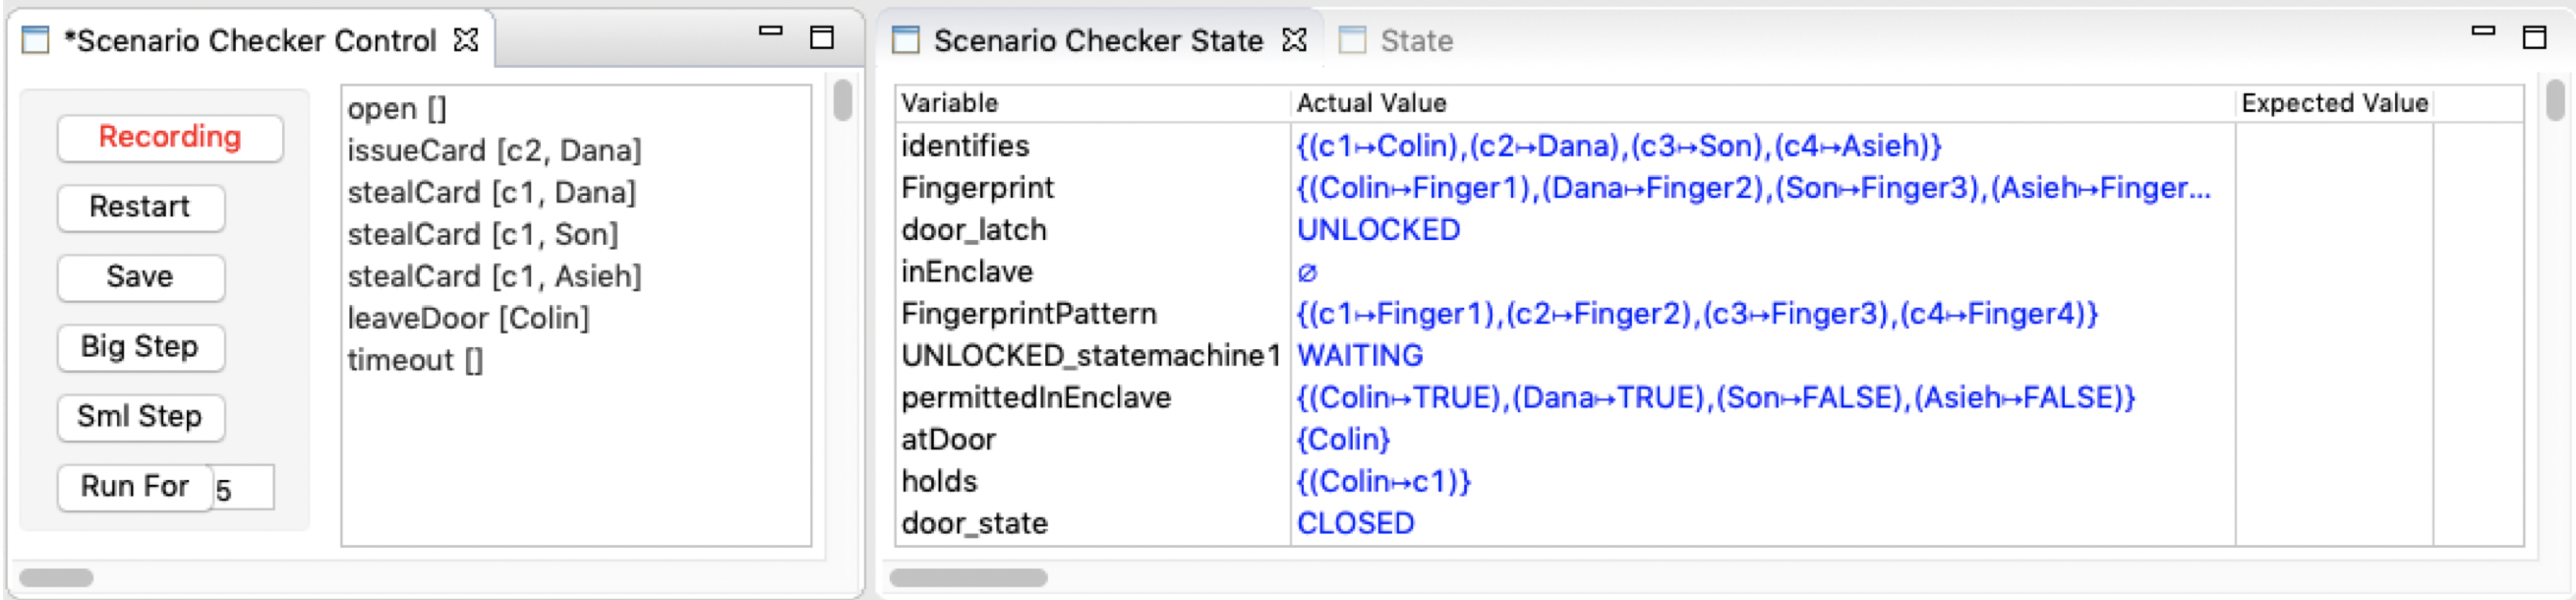
\includegraphics[width=512]{figures/recording}
	\else
	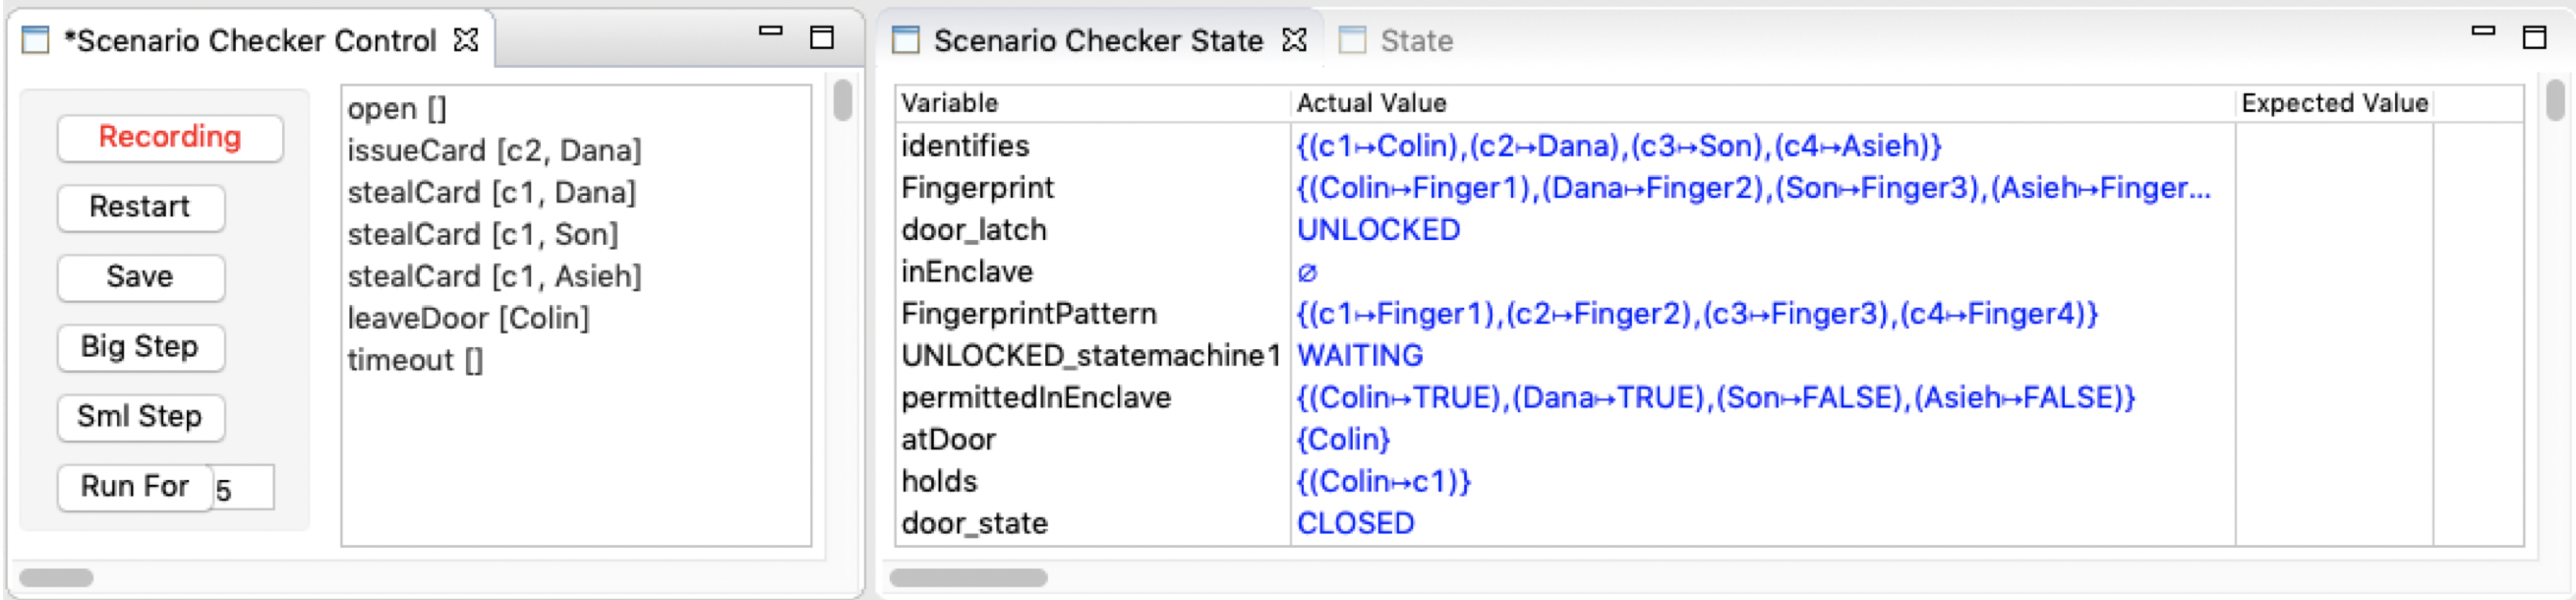
\includegraphics[width=0.9\textwidth]{figures/recording}
	\fi
	\caption{Recording}
	\label{fig:recording}
\end{figure}

\subsection{Re-playing a Scenario}
\label{sec:playback}

With the Scenario Checker in playback mode (see Replay button in Section~\ref{fig:recording}), the execution of events is taken from the scenario oracle file being replayed.
The user should not try to control the execution of events and an information message will be displayed if she attempts to select events from the Scenario Checker Control Panel. 
(Note that it is not possible to prevent other animation plug-ins (including the ProB `Events' view) from executing events but this would most likely make the scenario fail. 
The user presses the Big Step button to tell the Scenario Checker to execute the next recorded external event followed by any enabled internal events (similar to in recording mode).
The Scenario Checker then updates the Scenario Checker State view to show the state of any non-private variables that have changed state.
The expected value from the recording is shown and any differences are highlighted in red.
At any point, the playback can be stopped and an alternative ending can be recorded.

In playback mode, the Scenario Checker Control Panel buttons have the following function:
\begin{itemize}
	\item \textbf{Big Step}  Executes events until completion of the next big step. The external event is taken from the recording. If, after executing the external event, any internal events are enabled, one will be executed at random and according to any priority that has been defined in the model (see section~\ref{sec:concepts}). Firing of internal events will continue in this way until none are enabled or a loop is detected. (A loop is detected when the same event has already been executed in this run to completion).
	\item \textbf{Small Step}  Do not use in playback mode.
	\item \textbf{Run For..}   Do not use in playback mode.
	\item \textbf{Restart}  Discards the current scenario execution and restarts the same recorded scenario animation from the INITIALISATION. 
	\item \textbf{Save}  Saves the current scenario execution and continues without interruption still in playback. This enables common prefixes to be saved as partial scenarios for later completion. The scenario is saved in a folder called `Oracle' inside the Event-B project. The filename is automatically constructed from the machine name and a timestamp with the extension, `oracle'. 
	\item \textbf{Replay}  Discards the current scenario execution and restarts the same recorded scenario animation from the INITIALISATION. (i.e. same as Restart)
	\item \textbf{Stop}  Switches to recording mode. The scenario execution is left in whatever state it was during the playback. This allows multiple alternative scenarios to be recorded using a common recorded prefix.
\end{itemize}

In playback mode, the next external event in the recorded scenario (i.e. the event that will be executed when the big step button is next pressed) is highlighted in the list of enabled external events in the Scenario Checker Control Panel.

In playback mode the Scenario Checker View displays the current value of any non-private variables that have changed value since the last step.
The Expected value column displays the corresponding value from the recorded scenario for comparison.
If the values are the same the current value is displayed in green. 
If the values differ the current value is displayed in red.

When all steps in the recorded scenario have been played, the Scenario Checker automatically switches to recording mode without disturbing the current state of the scenario execution. This allows a the scenario to be extended to make a new, longer recorded scenario.

\begin{figure}[!htbp]
	\centering
	\ifplastex
	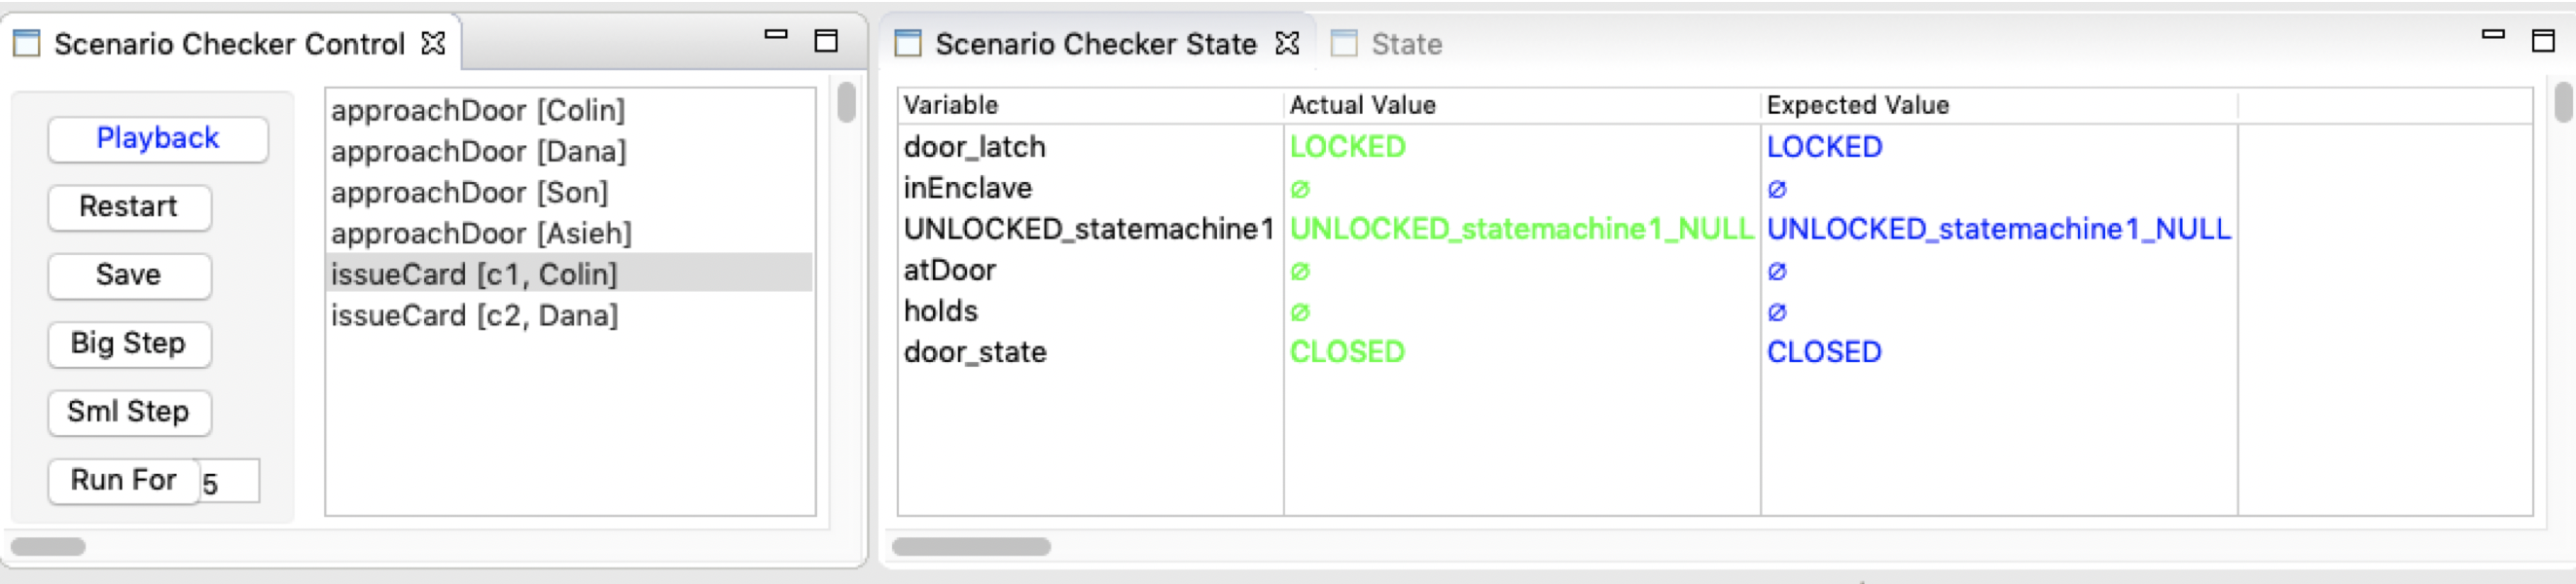
\includegraphics[width=512]{figures/playback}
	\else
	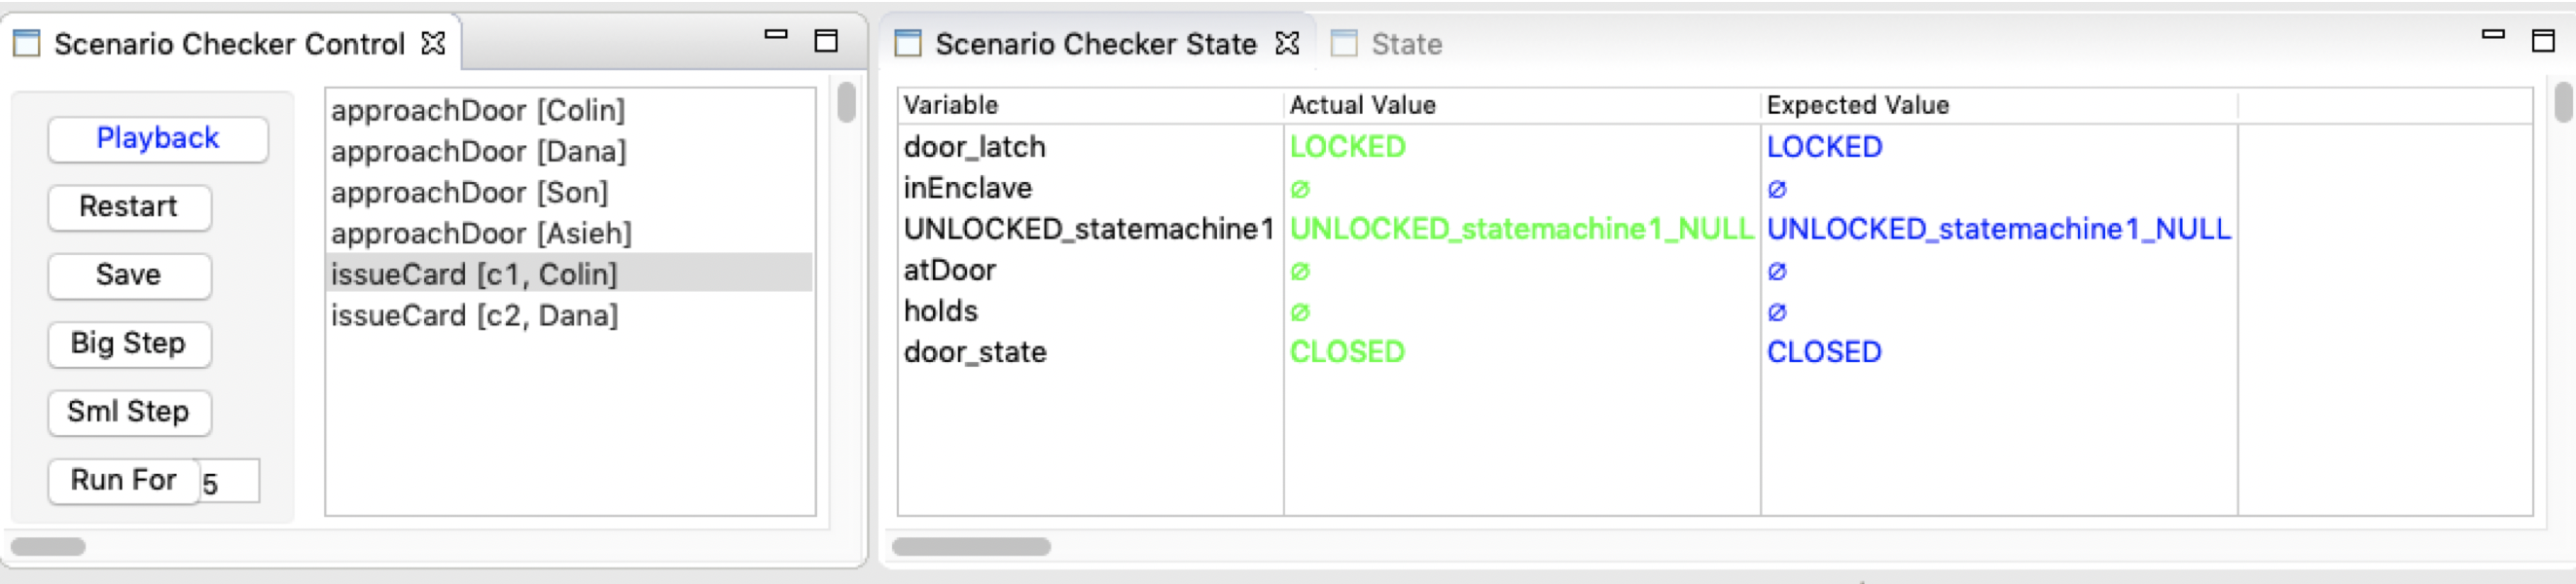
\includegraphics[width=0.9\textwidth]{figures/playback}
	\fi
	\caption{Playback}
	\label{fig:playback}
\end{figure}
%%% Local Variables:
%%% mode: latex
%%% TeX-master: "user_manual"
%%% End:


\section{Reference}
\label{sec:reference}

\subsection{Scenario Checker Console Messages}
\label{sec:consoleMessages}

The Scenario Checker Console displays the following messages:
(Placeholders shown in angle brackets \texttt{<xxx>} will be replaced with actual names etc.).
\begin{itemize}
	\item \texttt{Checking <machine name>} - when the scenario checker is first started or started after stopping.
	\item \texttt{Restarted} - when the scenario checker is restarted without stopping.
	\item \texttt{Stopped} - when the scenario checker is stopped.
	\item \texttt{Can not run until context is set up} - if a step is attempted when the ProB setup operation is enabled.
	\item \texttt{saved <recording name>} - after the scenario is saved.
	\item \texttt{mode changed to PLAYBACK} - after the mode has been changed to playback.
	\item \texttt{mode changed to RECORDING} - after the mode has been changed to recording.
	\item \texttt{BigStep - fired [ext] <event signature>} when the Big Step button is pressed (or an event fired from the list of enabled external events) and the event is fired successfully. (Note that it is also possible to fire an internal event if the previous big step aborted. In which case, [ext] is replaced by [int]). After this message is displayed the following messages will be displayed indented as part of the Big Step run.
	\begin{itemize}
		\item \texttt{- fired [int] <event signature>} when an internal event is successfully fired
		\item \texttt{- Big step ran to completion} when no internal events are enabled	
		\item \texttt{- Big step aborted due to deadlock} when no events are enabled
		\item \texttt{- Big step aborted due to loop on <event signature>} when the event shown has already been fired a number of times during this Big Step.	
	\end{itemize}
	\item \texttt{Small step - <event signature>} - when the Small Step button is pressed and an event is fired.
	\item \texttt{Small step aborted - nothing enabled} - when the Small Step button is pressed but no events are enabled.
	\item \texttt{Run For - Run terminated after <\#done> of <\#ticks> ticks due to lack of progress} - when the Run For button is pressed but a lack of progress is reported.
	\item \texttt{Run For - Completed all <\#done> ticks} - when the Run For button is pressed and completed
\end{itemize}

The following exceptional error messages indicate that ProB has not behaved as expected:
\begin{itemize}
	\item \texttt{The Scenario Checker aborted because ProB appears to have stopped animating the machine (i.e. sent null)}
	\item \texttt{The Scenario Checker aborted because ProB appears to be animating a different machine: <machine name>}
	\item \texttt{Exception in ProB while excecuting operation <event signature>}
\end{itemize}

%%% Local Variables:
%%% mode: latex
%%% TeX-master: "user_manual"
%%% End:


%\section{Samples}
\label{sec:samples}


%%% Local Variables:
%%% mode: latex
%%% TeX-master: "user_manual"
%%% End:


\ifplastex
\section{Legal}
\label{sec:legal}

\subsection{EPL Software User Agreement}
\label{sec:user-agreement}


Eclipse Public License - v 2.0

THE ACCOMPANYING PROGRAM IS PROVIDED UNDER THE TERMS OF THIS ECLIPSE
PUBLIC LICENSE ("AGREEMENT"). ANY USE, REPRODUCTION OR DISTRIBUTION
OF THE PROGRAM CONSTITUTES RECIPIENT'S ACCEPTANCE OF THIS AGREEMENT.

1. DEFINITIONS

"Contribution" means:

a) in the case of the initial Contributor, the initial content
Distributed under this Agreement, and

b) in the case of each subsequent Contributor:

i) changes to the Program, and

ii) additions to the Program;

where such changes and/or additions to the Program originate from
and are Distributed by that particular Contributor. A Contribution
"originates" from a Contributor if it was added to the Program by
such Contributor itself or anyone acting on such Contributor's behalf.
Contributions do not include changes or additions to the Program that
are not Modified Works.

"Contributor" means any person or entity that Distributes the Program.

"Licensed Patents" mean patent claims licensable by a Contributor which
are necessarily infringed by the use or sale of its Contribution alone
or when combined with the Program.

"Program" means the Contributions Distributed in accordance with this
Agreement.

"Recipient" means anyone who receives the Program under this Agreement
or any Secondary License (as applicable), including Contributors.

"Derivative Works" shall mean any work, whether in Source Code or other
form, that is based on (or derived from) the Program and for which the
editorial revisions, annotations, elaborations, or other modifications
represent, as a whole, an original work of authorship.

"Modified Works" shall mean any work in Source Code or other form that
results from an addition to, deletion from, or modification of the
contents of the Program, including, for purposes of clarity any new file
in Source Code form that contains any contents of the Program. Modified
Works shall not include works that contain only declarations,
interfaces, types, classes, structures, or files of the Program solely
in each case in order to link to, bind by name, or subclass the Program
or Modified Works thereof.

"Distribute" means the acts of a) distributing or b) making available
in any manner that enables the transfer of a copy.

"Source Code" means the form of a Program preferred for making
modifications, including but not limited to software source code,
documentation source, and configuration files.

"Secondary License" means either the GNU General Public License,
Version 2.0, or any later versions of that license, including any
exceptions or additional permissions as identified by the initial
Contributor.

2. GRANT OF RIGHTS

a) Subject to the terms of this Agreement, each Contributor hereby
grants Recipient a non-exclusive, worldwide, royalty-free copyright
license to reproduce, prepare Derivative Works of, publicly display,
publicly perform, Distribute and sublicense the Contribution of such
Contributor, if any, and such Derivative Works.

b) Subject to the terms of this Agreement, each Contributor hereby
grants Recipient a non-exclusive, worldwide, royalty-free patent
license under Licensed Patents to make, use, sell, offer to sell,
import and otherwise transfer the Contribution of such Contributor,
if any, in Source Code or other form. This patent license shall
apply to the combination of the Contribution and the Program if, at
the time the Contribution is added by the Contributor, such addition
of the Contribution causes such combination to be covered by the
Licensed Patents. The patent license shall not apply to any other
combinations which include the Contribution. No hardware per se is
licensed hereunder.

c) Recipient understands that although each Contributor grants the
licenses to its Contributions set forth herein, no assurances are
provided by any Contributor that the Program does not infringe the
patent or other intellectual property rights of any other entity.
Each Contributor disclaims any liability to Recipient for claims
brought by any other entity based on infringement of intellectual
property rights or otherwise. As a condition to exercising the
rights and licenses granted hereunder, each Recipient hereby
assumes sole responsibility to secure any other intellectual
property rights needed, if any. For example, if a third party
patent license is required to allow Recipient to Distribute the
Program, it is Recipient's responsibility to acquire that license
before distributing the Program.

d) Each Contributor represents that to its knowledge it has
sufficient copyright rights in its Contribution, if any, to grant
the copyright license set forth in this Agreement.

e) Notwithstanding the terms of any Secondary License, no
Contributor makes additional grants to any Recipient (other than
those set forth in this Agreement) as a result of such Recipient's
receipt of the Program under the terms of a Secondary License
(if permitted under the terms of Section 3).

3. REQUIREMENTS

3.1 If a Contributor Distributes the Program in any form, then:

a) the Program must also be made available as Source Code, in
accordance with section 3.2, and the Contributor must accompany
the Program with a statement that the Source Code for the Program
is available under this Agreement, and informs Recipients how to
obtain it in a reasonable manner on or through a medium customarily
used for software exchange; and

b) the Contributor may Distribute the Program under a license
different than this Agreement, provided that such license:

i) effectively disclaims on behalf of all other Contributors all
warranties and conditions, express and implied, including
warranties or conditions of title and non-infringement, and
implied warranties or conditions of merchantability and fitness
for a particular purpose;

ii) effectively excludes on behalf of all other Contributors all
liability for damages, including direct, indirect, special,
incidental and consequential damages, such as lost profits;

iii) does not attempt to limit or alter the recipients' rights
in the Source Code under section 3.2; and

iv) requires any subsequent distribution of the Program by any
party to be under a license that satisfies the requirements
of this section 3.

3.2 When the Program is Distributed as Source Code:

a) it must be made available under this Agreement, or if the
Program (i) is combined with other material in a separate file or
files made available under a Secondary License, and (ii) the initial
Contributor attached to the Source Code the notice described in
Exhibit A of this Agreement, then the Program may be made available
under the terms of such Secondary Licenses, and

b) a copy of this Agreement must be included with each copy of
the Program.

3.3 Contributors may not remove or alter any copyright, patent,
trademark, attribution notices, disclaimers of warranty, or limitations
of liability ("notices") contained within the Program from any copy of
the Program which they Distribute, provided that Contributors may add
their own appropriate notices.

4. COMMERCIAL DISTRIBUTION

Commercial distributors of software may accept certain responsibilities
with respect to end users, business partners and the like. While this
license is intended to facilitate the commercial use of the Program,
the Contributor who includes the Program in a commercial product
offering should do so in a manner which does not create potential
liability for other Contributors. Therefore, if a Contributor includes
the Program in a commercial product offering, such Contributor
("Commercial Contributor") hereby agrees to defend and indemnify every
other Contributor ("Indemnified Contributor") against any losses,
damages and costs (collectively "Losses") arising from claims, lawsuits
and other legal actions brought by a third party against the Indemnified
Contributor to the extent caused by the acts or omissions of such
Commercial Contributor in connection with its distribution of the Program
in a commercial product offering. The obligations in this section do not
apply to any claims or Losses relating to any actual or alleged
intellectual property infringement. In order to qualify, an Indemnified
Contributor must: a) promptly notify the Commercial Contributor in
writing of such claim, and b) allow the Commercial Contributor to control,
and cooperate with the Commercial Contributor in, the defense and any
related settlement negotiations. The Indemnified Contributor may
participate in any such claim at its own expense.

For example, a Contributor might include the Program in a commercial
product offering, Product X. That Contributor is then a Commercial
Contributor. If that Commercial Contributor then makes performance
claims, or offers warranties related to Product X, those performance
claims and warranties are such Commercial Contributor's responsibility
alone. Under this section, the Commercial Contributor would have to
defend claims against the other Contributors related to those performance
claims and warranties, and if a court requires any other Contributor to
pay any damages as a result, the Commercial Contributor must pay
those damages.

5. NO WARRANTY

EXCEPT AS EXPRESSLY SET FORTH IN THIS AGREEMENT, AND TO THE EXTENT
PERMITTED BY APPLICABLE LAW, THE PROGRAM IS PROVIDED ON AN "AS IS"
BASIS, WITHOUT WARRANTIES OR CONDITIONS OF ANY KIND, EITHER EXPRESS OR
IMPLIED INCLUDING, WITHOUT LIMITATION, ANY WARRANTIES OR CONDITIONS OF
TITLE, NON-INFRINGEMENT, MERCHANTABILITY OR FITNESS FOR A PARTICULAR
PURPOSE. Each Recipient is solely responsible for determining the
appropriateness of using and distributing the Program and assumes all
risks associated with its exercise of rights under this Agreement,
including but not limited to the risks and costs of program errors,
compliance with applicable laws, damage to or loss of data, programs
or equipment, and unavailability or interruption of operations.

6. DISCLAIMER OF LIABILITY

EXCEPT AS EXPRESSLY SET FORTH IN THIS AGREEMENT, AND TO THE EXTENT
PERMITTED BY APPLICABLE LAW, NEITHER RECIPIENT NOR ANY CONTRIBUTORS
SHALL HAVE ANY LIABILITY FOR ANY DIRECT, INDIRECT, INCIDENTAL, SPECIAL,
EXEMPLARY, OR CONSEQUENTIAL DAMAGES (INCLUDING WITHOUT LIMITATION LOST
PROFITS), HOWEVER CAUSED AND ON ANY THEORY OF LIABILITY, WHETHER IN
CONTRACT, STRICT LIABILITY, OR TORT (INCLUDING NEGLIGENCE OR OTHERWISE)
ARISING IN ANY WAY OUT OF THE USE OR DISTRIBUTION OF THE PROGRAM OR THE
EXERCISE OF ANY RIGHTS GRANTED HEREUNDER, EVEN IF ADVISED OF THE
POSSIBILITY OF SUCH DAMAGES.

7. GENERAL

If any provision of this Agreement is invalid or unenforceable under
applicable law, it shall not affect the validity or enforceability of
the remainder of the terms of this Agreement, and without further
action by the parties hereto, such provision shall be reformed to the
minimum extent necessary to make such provision valid and enforceable.

If Recipient institutes patent litigation against any entity
(including a cross-claim or counterclaim in a lawsuit) alleging that the
Program itself (excluding combinations of the Program with other software
or hardware) infringes such Recipient's patent(s), then such Recipient's
rights granted under Section 2(b) shall terminate as of the date such
litigation is filed.

All Recipient's rights under this Agreement shall terminate if it
fails to comply with any of the material terms or conditions of this
Agreement and does not cure such failure in a reasonable period of
time after becoming aware of such noncompliance. If all Recipient's
rights under this Agreement terminate, Recipient agrees to cease use
and distribution of the Program as soon as reasonably practicable.
However, Recipient's obligations under this Agreement and any licenses
granted by Recipient relating to the Program shall continue and survive.

Everyone is permitted to copy and distribute copies of this Agreement,
but in order to avoid inconsistency the Agreement is copyrighted and
may only be modified in the following manner. The Agreement Steward
reserves the right to publish new versions (including revisions) of
this Agreement from time to time. No one other than the Agreement
Steward has the right to modify this Agreement. The Eclipse Foundation
is the initial Agreement Steward. The Eclipse Foundation may assign the
responsibility to serve as the Agreement Steward to a suitable separate
entity. Each new version of the Agreement will be given a distinguishing
version number. The Program (including Contributions) may always be
Distributed subject to the version of the Agreement under which it was
received. In addition, after a new version of the Agreement is published,
Contributor may elect to Distribute the Program (including its
Contributions) under the new version.

Except as expressly stated in Sections 2(a) and 2(b) above, Recipient
receives no rights or licenses to the intellectual property of any
Contributor under this Agreement, whether expressly, by implication,
estoppel or otherwise. All rights in the Program not expressly granted
under this Agreement are reserved. Nothing in this Agreement is intended
to be enforceable by any entity that is not a Contributor or Recipient.
No third-party beneficiary rights are created under this Agreement.

Exhibit A - Form of Secondary Licenses Notice

"This Source Code may also be made available under the following 
Secondary Licenses when the conditions for such availability set forth 
in the Eclipse Public License, v. 2.0 are satisfied: {name license(s),
	version(s), and exceptions or additional permissions here}."

Simply including a copy of this Agreement, including this Exhibit A
is not sufficient to license the Source Code under Secondary Licenses.

If it is not possible or desirable to put the notice in a particular
file, then You may include the notice in a location (such as a LICENSE
file in a relevant directory) where a recipient would be likely to
look for such a notice.

You may add additional accurate notices of copyright ownership.


%%% Local Variables:
%%% mode: latex
%%% TeX-master: "user_manual"
%%% End:

\else
  \ifstandalone
  \section{Legal}
  \label{sec:legal}

  \subsection{EPL Software User Agreement}
  \label{sec:user-agreement}

  
Eclipse Public License - v 2.0

THE ACCOMPANYING PROGRAM IS PROVIDED UNDER THE TERMS OF THIS ECLIPSE
PUBLIC LICENSE ("AGREEMENT"). ANY USE, REPRODUCTION OR DISTRIBUTION
OF THE PROGRAM CONSTITUTES RECIPIENT'S ACCEPTANCE OF THIS AGREEMENT.

1. DEFINITIONS

"Contribution" means:

a) in the case of the initial Contributor, the initial content
Distributed under this Agreement, and

b) in the case of each subsequent Contributor:

i) changes to the Program, and

ii) additions to the Program;

where such changes and/or additions to the Program originate from
and are Distributed by that particular Contributor. A Contribution
"originates" from a Contributor if it was added to the Program by
such Contributor itself or anyone acting on such Contributor's behalf.
Contributions do not include changes or additions to the Program that
are not Modified Works.

"Contributor" means any person or entity that Distributes the Program.

"Licensed Patents" mean patent claims licensable by a Contributor which
are necessarily infringed by the use or sale of its Contribution alone
or when combined with the Program.

"Program" means the Contributions Distributed in accordance with this
Agreement.

"Recipient" means anyone who receives the Program under this Agreement
or any Secondary License (as applicable), including Contributors.

"Derivative Works" shall mean any work, whether in Source Code or other
form, that is based on (or derived from) the Program and for which the
editorial revisions, annotations, elaborations, or other modifications
represent, as a whole, an original work of authorship.

"Modified Works" shall mean any work in Source Code or other form that
results from an addition to, deletion from, or modification of the
contents of the Program, including, for purposes of clarity any new file
in Source Code form that contains any contents of the Program. Modified
Works shall not include works that contain only declarations,
interfaces, types, classes, structures, or files of the Program solely
in each case in order to link to, bind by name, or subclass the Program
or Modified Works thereof.

"Distribute" means the acts of a) distributing or b) making available
in any manner that enables the transfer of a copy.

"Source Code" means the form of a Program preferred for making
modifications, including but not limited to software source code,
documentation source, and configuration files.

"Secondary License" means either the GNU General Public License,
Version 2.0, or any later versions of that license, including any
exceptions or additional permissions as identified by the initial
Contributor.

2. GRANT OF RIGHTS

a) Subject to the terms of this Agreement, each Contributor hereby
grants Recipient a non-exclusive, worldwide, royalty-free copyright
license to reproduce, prepare Derivative Works of, publicly display,
publicly perform, Distribute and sublicense the Contribution of such
Contributor, if any, and such Derivative Works.

b) Subject to the terms of this Agreement, each Contributor hereby
grants Recipient a non-exclusive, worldwide, royalty-free patent
license under Licensed Patents to make, use, sell, offer to sell,
import and otherwise transfer the Contribution of such Contributor,
if any, in Source Code or other form. This patent license shall
apply to the combination of the Contribution and the Program if, at
the time the Contribution is added by the Contributor, such addition
of the Contribution causes such combination to be covered by the
Licensed Patents. The patent license shall not apply to any other
combinations which include the Contribution. No hardware per se is
licensed hereunder.

c) Recipient understands that although each Contributor grants the
licenses to its Contributions set forth herein, no assurances are
provided by any Contributor that the Program does not infringe the
patent or other intellectual property rights of any other entity.
Each Contributor disclaims any liability to Recipient for claims
brought by any other entity based on infringement of intellectual
property rights or otherwise. As a condition to exercising the
rights and licenses granted hereunder, each Recipient hereby
assumes sole responsibility to secure any other intellectual
property rights needed, if any. For example, if a third party
patent license is required to allow Recipient to Distribute the
Program, it is Recipient's responsibility to acquire that license
before distributing the Program.

d) Each Contributor represents that to its knowledge it has
sufficient copyright rights in its Contribution, if any, to grant
the copyright license set forth in this Agreement.

e) Notwithstanding the terms of any Secondary License, no
Contributor makes additional grants to any Recipient (other than
those set forth in this Agreement) as a result of such Recipient's
receipt of the Program under the terms of a Secondary License
(if permitted under the terms of Section 3).

3. REQUIREMENTS

3.1 If a Contributor Distributes the Program in any form, then:

a) the Program must also be made available as Source Code, in
accordance with section 3.2, and the Contributor must accompany
the Program with a statement that the Source Code for the Program
is available under this Agreement, and informs Recipients how to
obtain it in a reasonable manner on or through a medium customarily
used for software exchange; and

b) the Contributor may Distribute the Program under a license
different than this Agreement, provided that such license:

i) effectively disclaims on behalf of all other Contributors all
warranties and conditions, express and implied, including
warranties or conditions of title and non-infringement, and
implied warranties or conditions of merchantability and fitness
for a particular purpose;

ii) effectively excludes on behalf of all other Contributors all
liability for damages, including direct, indirect, special,
incidental and consequential damages, such as lost profits;

iii) does not attempt to limit or alter the recipients' rights
in the Source Code under section 3.2; and

iv) requires any subsequent distribution of the Program by any
party to be under a license that satisfies the requirements
of this section 3.

3.2 When the Program is Distributed as Source Code:

a) it must be made available under this Agreement, or if the
Program (i) is combined with other material in a separate file or
files made available under a Secondary License, and (ii) the initial
Contributor attached to the Source Code the notice described in
Exhibit A of this Agreement, then the Program may be made available
under the terms of such Secondary Licenses, and

b) a copy of this Agreement must be included with each copy of
the Program.

3.3 Contributors may not remove or alter any copyright, patent,
trademark, attribution notices, disclaimers of warranty, or limitations
of liability ("notices") contained within the Program from any copy of
the Program which they Distribute, provided that Contributors may add
their own appropriate notices.

4. COMMERCIAL DISTRIBUTION

Commercial distributors of software may accept certain responsibilities
with respect to end users, business partners and the like. While this
license is intended to facilitate the commercial use of the Program,
the Contributor who includes the Program in a commercial product
offering should do so in a manner which does not create potential
liability for other Contributors. Therefore, if a Contributor includes
the Program in a commercial product offering, such Contributor
("Commercial Contributor") hereby agrees to defend and indemnify every
other Contributor ("Indemnified Contributor") against any losses,
damages and costs (collectively "Losses") arising from claims, lawsuits
and other legal actions brought by a third party against the Indemnified
Contributor to the extent caused by the acts or omissions of such
Commercial Contributor in connection with its distribution of the Program
in a commercial product offering. The obligations in this section do not
apply to any claims or Losses relating to any actual or alleged
intellectual property infringement. In order to qualify, an Indemnified
Contributor must: a) promptly notify the Commercial Contributor in
writing of such claim, and b) allow the Commercial Contributor to control,
and cooperate with the Commercial Contributor in, the defense and any
related settlement negotiations. The Indemnified Contributor may
participate in any such claim at its own expense.

For example, a Contributor might include the Program in a commercial
product offering, Product X. That Contributor is then a Commercial
Contributor. If that Commercial Contributor then makes performance
claims, or offers warranties related to Product X, those performance
claims and warranties are such Commercial Contributor's responsibility
alone. Under this section, the Commercial Contributor would have to
defend claims against the other Contributors related to those performance
claims and warranties, and if a court requires any other Contributor to
pay any damages as a result, the Commercial Contributor must pay
those damages.

5. NO WARRANTY

EXCEPT AS EXPRESSLY SET FORTH IN THIS AGREEMENT, AND TO THE EXTENT
PERMITTED BY APPLICABLE LAW, THE PROGRAM IS PROVIDED ON AN "AS IS"
BASIS, WITHOUT WARRANTIES OR CONDITIONS OF ANY KIND, EITHER EXPRESS OR
IMPLIED INCLUDING, WITHOUT LIMITATION, ANY WARRANTIES OR CONDITIONS OF
TITLE, NON-INFRINGEMENT, MERCHANTABILITY OR FITNESS FOR A PARTICULAR
PURPOSE. Each Recipient is solely responsible for determining the
appropriateness of using and distributing the Program and assumes all
risks associated with its exercise of rights under this Agreement,
including but not limited to the risks and costs of program errors,
compliance with applicable laws, damage to or loss of data, programs
or equipment, and unavailability or interruption of operations.

6. DISCLAIMER OF LIABILITY

EXCEPT AS EXPRESSLY SET FORTH IN THIS AGREEMENT, AND TO THE EXTENT
PERMITTED BY APPLICABLE LAW, NEITHER RECIPIENT NOR ANY CONTRIBUTORS
SHALL HAVE ANY LIABILITY FOR ANY DIRECT, INDIRECT, INCIDENTAL, SPECIAL,
EXEMPLARY, OR CONSEQUENTIAL DAMAGES (INCLUDING WITHOUT LIMITATION LOST
PROFITS), HOWEVER CAUSED AND ON ANY THEORY OF LIABILITY, WHETHER IN
CONTRACT, STRICT LIABILITY, OR TORT (INCLUDING NEGLIGENCE OR OTHERWISE)
ARISING IN ANY WAY OUT OF THE USE OR DISTRIBUTION OF THE PROGRAM OR THE
EXERCISE OF ANY RIGHTS GRANTED HEREUNDER, EVEN IF ADVISED OF THE
POSSIBILITY OF SUCH DAMAGES.

7. GENERAL

If any provision of this Agreement is invalid or unenforceable under
applicable law, it shall not affect the validity or enforceability of
the remainder of the terms of this Agreement, and without further
action by the parties hereto, such provision shall be reformed to the
minimum extent necessary to make such provision valid and enforceable.

If Recipient institutes patent litigation against any entity
(including a cross-claim or counterclaim in a lawsuit) alleging that the
Program itself (excluding combinations of the Program with other software
or hardware) infringes such Recipient's patent(s), then such Recipient's
rights granted under Section 2(b) shall terminate as of the date such
litigation is filed.

All Recipient's rights under this Agreement shall terminate if it
fails to comply with any of the material terms or conditions of this
Agreement and does not cure such failure in a reasonable period of
time after becoming aware of such noncompliance. If all Recipient's
rights under this Agreement terminate, Recipient agrees to cease use
and distribution of the Program as soon as reasonably practicable.
However, Recipient's obligations under this Agreement and any licenses
granted by Recipient relating to the Program shall continue and survive.

Everyone is permitted to copy and distribute copies of this Agreement,
but in order to avoid inconsistency the Agreement is copyrighted and
may only be modified in the following manner. The Agreement Steward
reserves the right to publish new versions (including revisions) of
this Agreement from time to time. No one other than the Agreement
Steward has the right to modify this Agreement. The Eclipse Foundation
is the initial Agreement Steward. The Eclipse Foundation may assign the
responsibility to serve as the Agreement Steward to a suitable separate
entity. Each new version of the Agreement will be given a distinguishing
version number. The Program (including Contributions) may always be
Distributed subject to the version of the Agreement under which it was
received. In addition, after a new version of the Agreement is published,
Contributor may elect to Distribute the Program (including its
Contributions) under the new version.

Except as expressly stated in Sections 2(a) and 2(b) above, Recipient
receives no rights or licenses to the intellectual property of any
Contributor under this Agreement, whether expressly, by implication,
estoppel or otherwise. All rights in the Program not expressly granted
under this Agreement are reserved. Nothing in this Agreement is intended
to be enforceable by any entity that is not a Contributor or Recipient.
No third-party beneficiary rights are created under this Agreement.

Exhibit A - Form of Secondary Licenses Notice

"This Source Code may also be made available under the following 
Secondary Licenses when the conditions for such availability set forth 
in the Eclipse Public License, v. 2.0 are satisfied: {name license(s),
	version(s), and exceptions or additional permissions here}."

Simply including a copy of this Agreement, including this Exhibit A
is not sufficient to license the Source Code under Secondary Licenses.

If it is not possible or desirable to put the notice in a particular
file, then You may include the notice in a location (such as a LICENSE
file in a relevant directory) where a recipient would be likely to
look for such a notice.

You may add additional accurate notices of copyright ownership.


%%% Local Variables:
%%% mode: latex
%%% TeX-master: "user_manual"
%%% End:

  \else
  \fi
\fi

%%% Local Variables:
%%% mode: latex
%%% TeX-master: "user_manual"
%%% End:


\end{document}

%%% Local Variables:
%%% mode: latex
%%% TeX-master: t
%%% End:
